\documentclass[french]{article}
\usepackage[T1]{fontenc}
\usepackage[utf8]{inputenc}
\usepackage[french]{babel}
\usepackage{amsmath}
\usepackage{mathtools}
\usepackage{color}
\usepackage[svgnames,dvipsnames]{xcolor} 
\usepackage{soul}
\usepackage{amssymb}
\usepackage{enumitem}
\usepackage{multicol}
\usepackage[left=2cm,right=2cm,top=2cm,bottom=2cm]{geometry}
\newcommand{\mathcolorbox}[2]{\colorbox{#1}{$\displaystyle #2$}}
\usepackage{pifont}
\usepackage{pst-all}
\usepackage{pstricks}
\usepackage{delarray}
\usepackage{setspace}
\usepackage{graphicx}
\usepackage{hyperref}
\usepackage{nicematrix}
\usepackage{listings}
\usepackage{float}

\hypersetup{
	colorlinks=true,
	linkcolor=blue,
	filecolor=magenta,      
	urlcolor=cyan,
	pdfpagemode=FullScreen,
}

\usepackage{amsthm}
\newtheorem*{Rem}{Remarque}

\newenvironment{conclusion}[1]{%
	\begin{center}\normalfont\textbf{Conclusion}\end{center}
	\begin{quotation} #1 \end{quotation}
}{%
	\vspace{1cm}
}

\newcommand\pythonstyle{\lstset{
	language=Python,
	basicstyle=\ttm,
	morekeywords={self},              % Add keywords here
	keywordstyle=\ttb\color{deepblue},
	emph={MyClass,__init__},          % Custom highlighting
	emphstyle=\ttb\color{deepred},    % Custom highlighting style
	stringstyle=\color{deepgreen},
	frame=tb,                         % Any extra options here
	showstringspaces=false
}}

\lstdefinestyle{Cpp}{
	language=C++,
	tabsize=3,
	basicstyle=\ttfamily,
	keywordstyle=\color{blue}\ttfamily,
	stringstyle=\color{red}\ttfamily,
	commentstyle=\color{green}\ttfamily,
	morecomment=[l][\color{magenta}]{\#}
}

\lstdefinestyle{Python}{
	language=Python,
	tabsize=3,
	basicstyle=\ttfamily,
	keywordstyle=\color{blue}\ttfamily,
	stringstyle=\color{red}\ttfamily,
	commentstyle=\color{green}\ttfamily,
	morecomment=[l][\color{magenta}]{\#}
}

\lstset{style=Cpp}

\setlength\parindent{0pt}
\usepackage[skip=2pt]{caption}

\usepackage{fontawesome}

\usepackage{lipsum}

\DeclareMathOperator*{\argmax}{argmax}
\DeclareMathOperator*{\argmin}{argmin}
\begin{document}
	LECOURTIER Frédérique \hfill \today
	\begin{center}
		\Large\textbf{{2_levelset}}
	\end{center}
	\tableofcontents
	\newpage
	\graphicspath{{images/1_introduction}}
	\section{Introduction} \label{levelset_intro}

On se place ici dans le contexte de la résolution d'EDP par des méthodes types PINNs. 

On cherche dans un premier temps à se concentrer sur le problème de Poisson avec conditions de Dirichlet défini par

\begin{equation*}
	\left\{\begin{aligned}
		&-\Delta u(X) = f(X) \quad \text{dans } \Omega, \\
		&u(X) = g(X) \quad \text{sur } \partial \Omega
	\end{aligned}\right.
\end{equation*}

La méthode PINNs standard consiste alors à chercher $\theta_u$ tel que
\begin{equation*}
	\theta_u = \argmin_{\theta} w_{r}\; J_{r}(\theta)+w_{bc}\; J_{bc}(\theta)
\end{equation*}
où $w_{r}$ et $w_{bc}$ sont les poids respectifs associés à
\begin{equation*}
	J_{r} = \int_\Omega (\Delta u_\theta+f)^2 \; \text{ et } \; J_{bc} = \int_{\partial\Omega} (u_\theta-g)^2.
\end{equation*}	

\begin{Rem}
	En pratique, on utilise une méthode de Monte-Carlo pour discrétiser les fonctions de coût par des processus aléatoires.
\end{Rem}

Dans ce contexte, l'idée reçue sur les PINNs est la suivante : 

\begin{center}
	\textbf{Comme il n'y a pas de maillage, c'est très facile de passer à des géométries complexes !}
\end{center}

Sauf que en pratique ce n'est pas si simple, en fait on va devoir trouver comment sampler (échantillonner) à l'intérieur de $\Omega$.

Dans le cas des géométries simples, on peut facilement trouver des méthodes permettant de sampler dans notre géométrie, c'est-à-dire récupérer un ensemble de points à l'intérieur de celle-ci.

\begin{figure}[H]
	\centering
	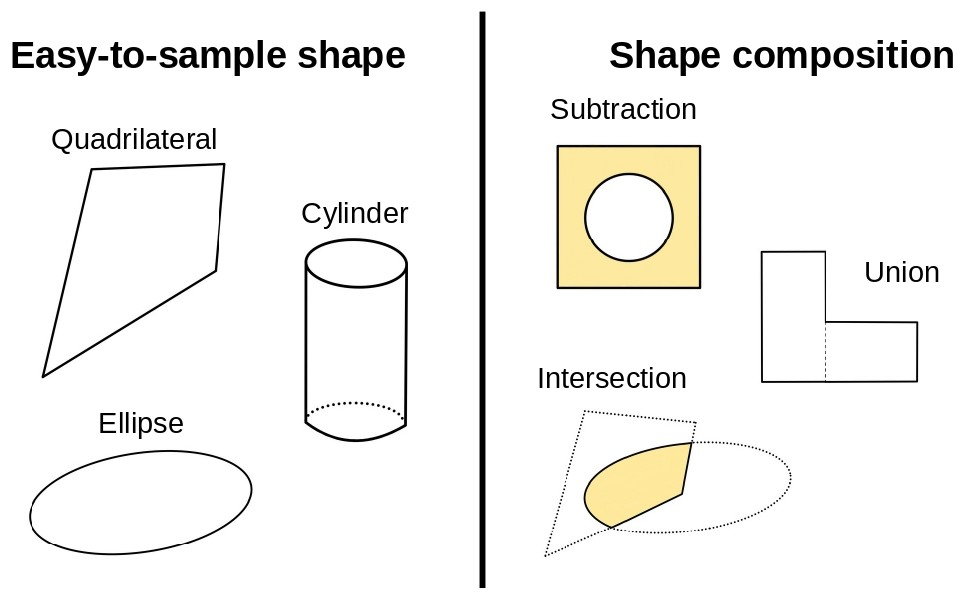
\includegraphics[width=0.6\linewidth]{simple_geom.jpg}
	\caption{Représentation de formes simples.}
\end{figure}

Comme on se place dans le contexte présenté en Section \hl{rajouter REF}, on considère des formes qui peuvent être beaucoup plus compliquée et on se heurte à un premier problème qui consiste à trouver comment sampler à l'intérieur de géométrie plus complexe.

On regroupe alors ce problème en deux approches principales : sampling par mapping ou sampling par levelset.

\begin{enumerate}[label=\textbullet]
	\item \textbf{Mapping :} Dans cette première approche, on considère un domaine simple $\Omega_0$, facile à sampler tel qu'un cercle. Cette méthode consiste à trouver une transformation $\phi$ tel que
	\begin{equation*}
		\Omega = \phi(\Omega_0)
	\end{equation*}
	où $\Omega$ est la géométrie cible.
	\begin{figure}[H]
		\centering
		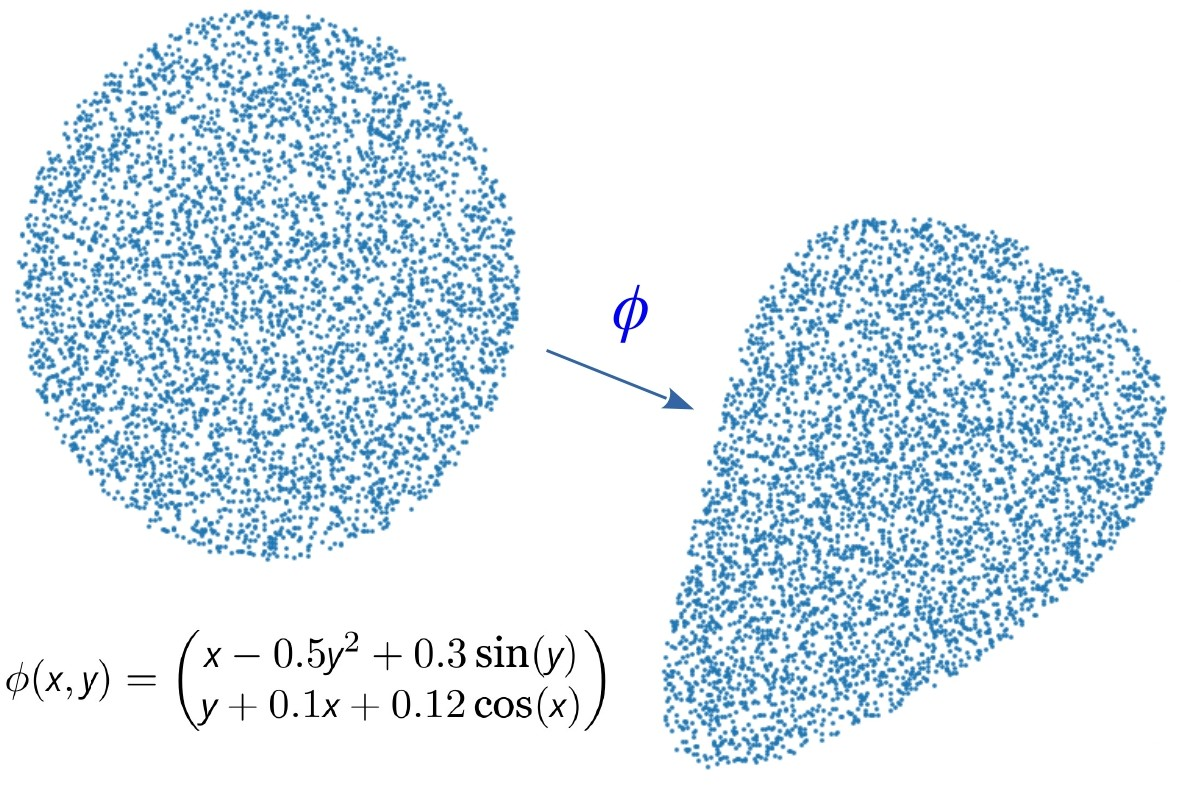
\includegraphics[width=0.4\linewidth]{complex_geom_mapping.jpg}
		\caption{Représentation d'un sampling par mapping.}
	\end{figure}

	\item \textbf{Levelset :} Dans cette seconde approche, on cherche à trouver une fonction levelset permettant de décrire notre géométrie.
	\begin{figure}[H]
		\centering
		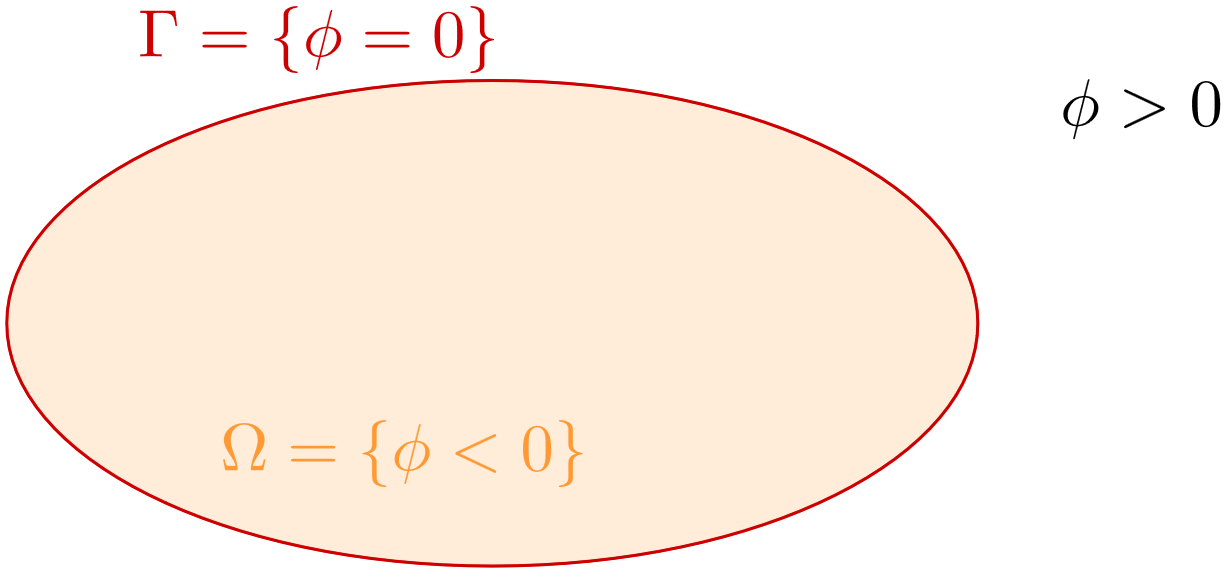
\includegraphics[width=0.3\linewidth]{complex_geom_levelset.png}
		\caption{Définition d'une fonction LevelSet.}
	\end{figure}
	Cette fonction est définie comme étant nulle sur le bord de notre domaine, strictement négative à l'intérieur et strictement positive à l'extérieur. Ainsi déterminer un sampling à l'intérieur de $\Omega$ revient seulement à déterminer des points tel que $\phi$ soit strictement négative.
\end{enumerate}

Dans le travail fait ici, on ne s'intéressera en fait que l'approche par LevelSet pour les raisons suivantes :
\begin{enumerate}[label=\textbullet]
	\item Dans notre contexte, on cherche à utiliser une méthode qui est en développement dans l'équipe Mimesis. Cette méthode appelée $\phi$-FEM (Section \hl{Rajouter ref}) est une méthode élément finie  non-conforme qui nécessite l'utilisation d'une fonction LevelSet. Ainsi, cette fonction Levelset sera utilisée pour sampler le domaine mais également dans la méthode $\phi$-FEM pour corriger et certifier les predcitions du PINNs.
	\item Ensuite, on s'est basé sur un papier \hl{Rajouter ref} qui permet d'imposer en dure les conditions au bord dans le PINNs en écrivant notre solution sous la forme
	\begin{equation*}
		u_\theta(X)=\phi(X)w_\theta(X)+g(X)
	\end{equation*}
	Ce papier semblait donner dans certains cas de meilleurs résultats qu'avec des PINNs standard.
	\begin{Rem}
		Ils présentent également des façons d'imposer des conditions de Neumann et de Robin mais on ne considérera ici qu le cas des conditions de Dirichlet.
	\end{Rem}
\end{enumerate}
Ainsi, on utilisera la fonction levelset pour générer un sampling dans notre géométrie, pour imposer les conditions en dure dans le PINNs mais également pour corriger et certifier les prédictions du PINNs en utilisant la méthode $\phi$-FEM.

\begin{Rem}
	Une fonction levelset naturelle est la Fonction Distance Signée. Cette fonction est totalement utilisable pour générer un sampling dans notre domaine. Cependant dans l'approche où on impose les conditions en dure, ses dérivées explosent trop pour obtenir des résultats satisfaisant. On se heurte alors au problème : Comment construire une fonction levelset suffisamment régulière pour pouvoir être utilisé pour imposer les conditions en dure ?
\end{Rem}

On cherche à présent à déterminer comment obtenir une fonction levelset pour des géométrie complexes. On distinguera alors deux approches :
\begin{enumerate}[label=\textbullet]
	\item Dans la première, on reprend le papier où sont imposés les conditions en dure et on utilise les théories d'approximation qui y sont proposées (Section \hl{rajouter REF}).
	\item Dans la seconde, on utilise une approche par apprentissage basé sur un second papier \hl{Rajouiter REF} (Section \hl{rajouter REF}).
\end{enumerate}
	\newpage
	\graphicspath{{images/2_maths_theory}}
	\section{Théorie d'approximation} \label{levelset_theory}
	\newpage
	\graphicspath{{images/3_learning}}
	\section{Apprentissage} \label{levelset_learning}
\end{document}